\begin{figure}[H]
	\centering
	\begin{tikzpicture}[baseline, scale=0.6]
	\pie[rotate=90, /tikz/nodes={text opacity=0,overlay}, color={yellow!40, blue!30}]{2/a, 98/b};
	\end{tikzpicture}
	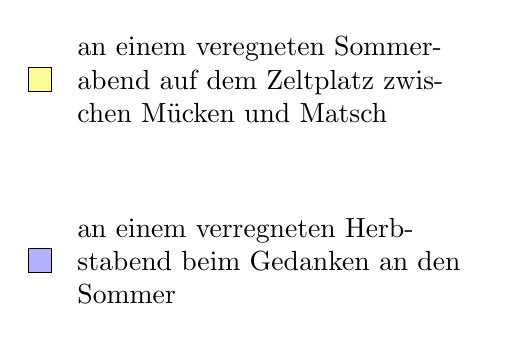
\begin{tikzpicture}[baseline]
	\draw [fill=yellow!40](0,1.0) rectangle (0.3,1.3);
	\node [text width=5cm,align=left, anchor=west] at (0.5,1.15) {an einem veregneten Sommerabend auf dem Zeltplatz zwischen Mücken und Matsch};
	\draw [fill=blue!30](0,-1.0) rectangle (0.3,-1.3);
	\node [text width=5cm,align=left, anchor=west] at (0.5,-1.15) {an einem verregneten Herbstabend beim Gedanken an den Sommer};
	\end{tikzpicture}
	\caption{Wann ein Zelt-Wochenende eine tolle Idee ist}
\end{figure}